% !TEX encoding = UTF-8 Unicode
% !TEX root = rapport.tex

\chapter{Les conséquences d'évolutions divergentes}
Du constat de la dichotomie dans l'intégration de la technologie par la société et par l'éducation, émerge un questionnement : quelles sont les conséquences de ce décalage pour les individus ?



\section{Des formations en inadéquation avec les besoins de la société} % de l'industrie ?
La faible intégration des \gls{ticLabel} dans l'éducation pose un certain nombre de problèmes quant à la pertinence des formations. En effet, les attentes de l'industrie et de la société quant aux compétences d'un individu comprennent la maitrise des \gls{ticLabel} ! Ces attentes se portent également sur les capacités à raisonner et à être créatif et de moins en moins sur les facultés de calcul ou sur la capacité à engranger des connaissances. Être capable d'accéder aux informations voulues rapidement devient alors essentiel dans un monde où internet fourni la plupart des connaissances mondiales.

Examinons alors les données du chômage des jeunes et ce que nous pouvons en déduire sur la pertinence de leur formation.

\subsection{Taux de chômage des jeunes}
Commençons tout d'abord par examiner les données du chômage des jeunes comparées aux données globales du chômage (voir figures \ref{chom} et \ref{chom_jeunes}). Comme nous pouvons le constater, le chômage des jeunes est en moyenne deux fois plus important que le taux général du chômage en Europe. Cette disparité a de nombreuses explications dont certaines économiques. Nous pensons néanmoins que les causes dues à une formation inadaptée ne sont pas négligeables. 

\begin{figure}[p]
\centering
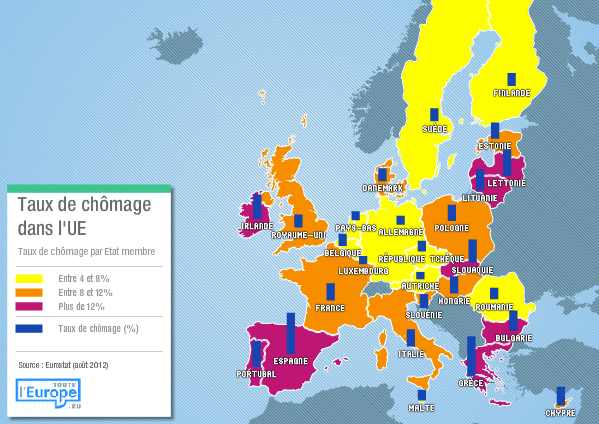
\includegraphics[width=0.98\linewidth]{figures/chom}
\caption{Taux de chômage dans l'UE en août 2012 \cite{chom}}
\label{chom}
\end{figure}
\begin{figure}[p]
\centering
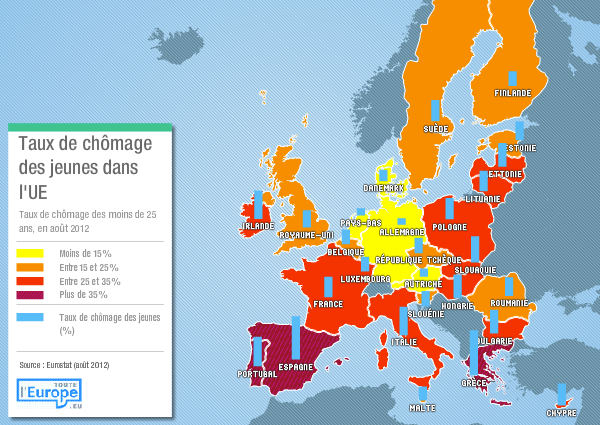
\includegraphics[width=0.98\linewidth]{figures/chom_jeunes}
\caption{Taux de chômage des jeunes dans l'UE en août 2012 \cite{chom_jeunes}}
\label{chom_jeunes}
\end{figure}

En effet, les formations dispensées ne sont pas fondamentalement différentes de celles du début du  \siecle{20} \cite{robinson2010paradigms} dans des contextes de révolution industrielle et du siècle des lumières. Cependant, les nouvelles technologies (machines, ordinateurs, automates\ldots) changent la donne ; de nos jours les machines remplacent les départs en retraite dans les industries ; les ordinateurs calculent bien plus efficacement que les humains ; la fiabilité des technologies dépasse de loin celle des humains.



\section{Les retombées imprévues de l'utilisation des technologies de la communication}

\subsection{Piège de Facebook pour les jeunes}



\section{Décrochages et échecs scolaires}
\subsection{La formation des étudiants en inadéquation avec leurs attentes}


\subsection{Hyperactivité chez les gamins qui ont juste besoin d'autre chose}
% auto-formation

